\documentclass[10pt, a4paper]{jreport}

\usepackage[dvipdfmx]{graphicx}
\usepackage{here}
\usepackage{comment}
\usepackage{otf}
\usepackage{framed}
\usepackage{longtable}

% 「関連図書」を「参考文献」に変換させる.
\renewcommand{\bibname}{参考文献}

\usepackage{listings}
\renewcommand{\lstlistingname}{ソースコード}
%\usepackage{color}
\lstset{%
  %language={C},
  basicstyle={\small},%
  identifierstyle={\small},%
  commentstyle={\small\itshape\color[rgb]{0,0.5,0}},%
  keywordstyle={\small\bfseries\color[rgb]{0,0,1}},%
  ndkeywordstyle={\small},%
  stringstyle={\small\ttfamily\color[rgb]{1,0,1}},
  frame={tb},
  breaklines=true,
  columns=[l]{fullflexible},%
  numbers=left,%
  xrightmargin=0zw,%
  xleftmargin=3zw,%
  numberstyle={\scriptsize},%
  stepnumber=1,
  numbersep=1zw,%
  lineskip=-0.5ex%
}

% \title{タイトル}
% \author{}
% \date{}

\begin{document}
% \maketitle

% ----------------------------------------------------------------------------------------------------
\tableofcontents

\chapter{はじめに}
\setcounter{page}{1}
インターネットの急速な普及に伴って,情報のアクセスが容易になり,我々の生活が豊かになった一方で,インターネットを悪用したサイバー犯罪が横行している.

サイバー犯罪は,サーバやアプリケーションの脆弱性を利用して,アクセス権限を要する情報を不正に入手したり,サーバに莫大な負荷をかけて,サービスに支障をきたしたりする行為のことである.サイバー犯罪の被害として,顧客の個人情報が流出したり,サービスが長期間,利用できなくなることなどが挙げられる.これらの被害は,サービスを利用する顧客にとっても,サービスを運営する企業にとっても大きな損失となるため,サイバー犯罪の被害を未然に防ぐことはもちろん,被害に遭った際に犯人を特定するための対策を講じることも重要である.

サイバー犯罪の犯人を特定する情報として,多くの場合,IPアドレスが用いられる.サイバー犯罪の被害を受けたサーバのログから,サイバー犯罪に該当するアクセスのIPアドレスを捜査し,インターネットサービスプロバイダに照会を要請することで,犯人の身元を特定することができる.

しかし,技術の進歩により,近年では,IPアドレスのみによる個人の特定は困難になってきている.VPNやTorを用いることで,インターネットサービスプロバイダから割り振られている本来のIPアドレスを秘匿化してインターネットに接続することができる.また,キャリアグレードNATの普及により,通常よりIPアドレスでの個人の特定が難しくなっていることも事実である.これらの技術についての詳細は,次章で後述する.

そこで,本論文では,サイバー犯罪が発生した際に,IPアドレス以外の方法で犯人を特定する手法について提案する.インターネット利用者が,サーバに送信する情報は複数挙げられるが,その中でもCookieに着目した特定システムを提案する.Cookieは,WebサーバがWebブラウザに対して,任意の文字列を記憶させるための仕組みである.サーバからCookieを保存するように指示されたブラウザは,以降,そのWebサイトに対して,記憶したCookieを送信するようになる.

Cookieを利用することで,サービスのログイン状態を記憶したり,ECサイトにおいて,ショッピングカートの中身を記憶させたりすることができる.一方で,アクセスしてきたユーザに,ユニークな文字列を発行し,Cookieとして保存させることで,過去にそのユーザがアクセスしてきたかどうかがわかるため,個人を特定するために用いられることもある.このように,Cookieはユーザを特定する十分な情報となり得る.

% ここに,この論文の章立ての説明を書く.
















%サイバー犯罪が起こった際に,IPアドレスなどで犯人を特定するが,最近では,キャリアグレードNATなどの技術の普及により,IPアドレスでの追跡は困難となっている.そこで,IPアドレス以外の情報,たとえばCookieなどを用いることで犯人を特定する手法について提案する.
\chapter{研究背景}
\section{IPアドレスによる特定の難しさ}
発信元のIPアドレスを特定することで,発信者の利用しているインターネットサービスプロバイダやキャリア,地域レベルの位置情報を取得できることが多い.サイバー犯罪が発生した際に,IPアドレスからインターネットサービスプロバイダを特定し,インターネットサービスプロバイダに照会を要請することで犯人を特定することができる.

しかし,技術の進歩により,IPアドレスによる個人の特定は困難であるケースも珍しくない.IPアドレスによる個人の特定が困難となる技術の代表例を以下に示す.

\subsection{キャリアグレードNAT}
キャリアグレードNATとは,インターネットサービスプロバイダなどが,ネットワークアドレス変換(NAT)を行う仕組みである.ネットワークアドレス変換とは,同一LAN内の各端末に割り振られたプライベートIPアドレスと,インターネットサービスプロバイダから割り振られたグローバルIPアドレスを変換するための仕組みである.IPv4アドレスの枯渇問題により,インターネットに接続する各端末すべてにグローバルIPアドレスを割り振ることは困難である.そこで,各端末には,グローバルIPアドレスの代わりに,プライベートIPアドレスを割り振り,インターネットに接続する際に,プライベートIPアドレスをグローバルIPアドレスに変換することで,LAN内の複数の端末を同じグローバルIPアドレスでインターネットに接続させることができる.ネットワークアドレス変換は,各家庭のLAN内で行われるが,これをインターネットサービスプロバイダ単位で行ったものがキャリアグレードNATである.

IPv4アドレスの枯渇問題を解消する手段として,キャリアグレードNATがしばしば利用されているが,同一のグローバルIPアドレスが,複数のインターネット利用者によって使用されるため,キャリアグレードNATを使用している場合は,IPアドレスによる個人の特定が困難となる.インターネットサービスプロバイダでは,キャリアグレードNATを利用した際のIPアドレスの変換テーブルを保持しているが,変換テーブルは,最新の約2ヶ月分しか記録されていないため,保存期間を過ぎると,IPアドレスによる特定ができなくなる.

\subsection{VPN}

\subsection{Tor}

\section{IPアドレスによる誤認逮捕}

\section{Cookieによる個人の特定}
IPアドレスによる個人の特定は困難であったり,誤認逮捕を招いたりする可能性があるため,サイバー犯罪において犯人を特定する情報としては,十分とはいえない.そこで,本論文では,Cookieによる個人の特定可能性に着目した.

Cookieとは,Webサーバが,Webブラウザに対して,任意の情報(文字列)を記憶させるための仕組みである.サーバからCookieを保存するように指示されたブラウザは,以降,そのWebサイトに対して,記憶したCookieを送信するようになる.

Cookieを利用することで,サービスのログイン状態を記憶したり,ECサイトにおいて,ショッピングカートの中身を記憶させたりすることができる.一方で,アクセスしてきたユーザに,ユニークな文字列を発行し,Cookieとして保存させることで,過去にそのユーザがアクセスしてきたかどうかを調べることができる.このように,Cookieはユーザを特定する十分な情報となり得る.

ブラウザがサーバに送信する情報として,使用している言語,ブラウザやOSの種類,バージョンなどが挙げられるが,これらは他のユーザと似たような情報となることが多い上,本来とは異なる情報を送信することも可能である.それに対して,Cookieは,サーバがブラウザに保存するように指示する値であるため,サーバがユニークな値を発行し,発行した値を記録しておくことができる.そのため,他のユーザと区別することができる上,ユーザが,サーバから指示された値とは異なるCookieを送信しても,詐称したことがわかる.よって,Cookieは,ブラウザがサーバに送信する情報の中でも,個人を特定できる可能性が高いことがわかる.

\section{SNSによる個人の特定}
%参考文献に出典をまとめる!
近年,多くのインターネット利用者がSNSを利用している.Twitter社が公開した"Q2 2017 Letter to Shareholders"によれば,2017年におけるTwitterの月間利用者数は3億2800万人である.また,Facebook社が公開した"Facebook Q2 2017 Results"によれば,2017年におけるFacebookの月間利用者数は約20億人である.SNSが発展した現代においては,世界中の人々が,SNSを通じてインターネットに自分の情報を発信しているといえる.

TwitterやFacebookなどのSNSには,多くの個人情報が保存されている.そのため,サイバー犯罪の犯人が利用しているSNSのアカウントを特定し,SNSを運営する企業に協力を依頼することで,犯人の身元を特定することは十分に可能であると考えられる.

最近の多くのWebサイト,とりわけニュースサイトやブログサイトでは,自身もしくは自社のサイトを読者に広めてもらうために,SNSのシェアボタンを設置していることが多い.SNSのシェアボタンのリソース(画像やスクリプトなど)を読み込むために,ブラウザはSNSのサイトに対してリクエストを送信するが,その際に,ユーザがそのSNSにログインした状態であれば,SNSのサーバにセッション情報を含むCookieを送信しているはずである.

したがって,SNSのシェアボタンを設置したサイトでサイバー犯罪が発生した際,犯人がそのSNSにログインした状態であれば,犯人のSNSのアカウントを特定することができる可能性が高いと考えられる.Cookieが個人を特定する情報となり得ることについては前述したが,SNSのCookieはサイバー犯罪の犯人を特定する上で非常に重要な情報であるといえる.

\section{犯人の不注意による逮捕事例}
SNSによる特定は,犯人がSNSにログインしていることが前提である.用心深い犯人であれば,サイバー犯罪を行う前にSNSからログアウトしているか,別のブラウザを使用しているであろう.

%出典を明記したい。書かれていることが曖昧な可能性がある
しかし,すべてのサイバー犯罪の犯人が,完全に証拠を残さずに犯罪を行うわけではない.実際に,Torを利用して児童ポルノを投稿した犯人が逮捕された事例がある.Torを使用することで発信元を隠蔽することができるが,逮捕された犯人は,Torの利用中に,不注意により通常のブラウザを使用したために発信元を特定されてしまった.このように,犯人の不注意によって逮捕されるケースもある.

SNSにおいて,利用を中断する度にログアウトするユーザは少数であると考えられる.ログインした状態でも通常のインターネットの使用に支障がないためである.よって,SNSにログインした状態で,そのSNSのシェアボタンが設置されたサイトにアクセスすることは十分に考えられる.犯人の不注意によりSNSのアカウントを特定することは,犯人の特定に大きく寄与するといえる.
















\chapter{研究方法}
\section{研究目的}
%第2章で書いたことをまとめる。こんな感じで
\begin{comment}
IPアドレスによる特定は難しい。誤認逮捕などもあるため問題である
↓
Cookieは個人を特定する上で重要な情報となり得る
↓
近年ではSNSが普及したことにより多くのユーザがSNSを利用するようになった
SNSは通常ログインしっぱなしであり、ログアウトすることはめったにない
↓
犯人がサイバー犯罪を行う際に、うっかりSNSにログインしたままである可能性がある
実際に、過去にはTorからサイバー犯罪を行った犯人が、うっかりふつうのブラウザを使ってしまったことで特定されてしまった
↓
SNSのシェアボタンに送信されたCookieを追跡することで、掲示板に書き込んだユーザを特定することができるのではないか
\end{comment}
第2章で述べたように,IPアドレスによる特定は困難である.そのため,サイバー犯罪の犯人を特定する際は,IPアドレスだけでなく,それ以外の情報を元に特定する手法が必要である.本論文では,Cookieが個人を特定できる可能性が高いことに着目した.また,近年においてSNSを利用するユーザが多く存在し,ログアウトする機会が少ないことから,サイバー犯罪において,犯人のSNSのアカウントを発見することが,犯人の特定に大きく寄与するのではないかと考えられる.最近では,SNSのシェアボタンを設置するWebサイトが多く見受けられる.SNSのシェアボタンを読み込む際に送信されたCookieを利用することで,サイバー犯罪の犯人を特定する手法を提案することを目的とする.

\section{提案手法}
SNSのシェアボタンを読み込む際に送信されたCookieから,個人をどの程度特定できるか実験するために,本研究では,匿名掲示板サイトとSNSサイトを用意した.










\chapter{実装}
\section{匿名掲示板}\label{sec: bbs}
本研究で使用した匿名掲示板は,インターネット上にフリーソフトウェアとして公開されているKENT-WEBのLIGHT BOARD(以下,LIGHT BOARD)である.この掲示板は,アカウント登録が不要で利用できる掲示板サイトである.名前の入力が必須となっているが,実名を入力する必要はなく,投稿毎に別の名前を入力することも可能であるため,匿名掲示板として利用することができる.

本研究では,LIGHT BOARDのソースプログラムをダウンロードし,改変したものを,自身のサーバで公開し実験を行った.実験で使用した匿名掲示板サイトを図\ref{fig: bbs_screenshot}に示す.

\begin{figure}[H]
	\begin{center}
		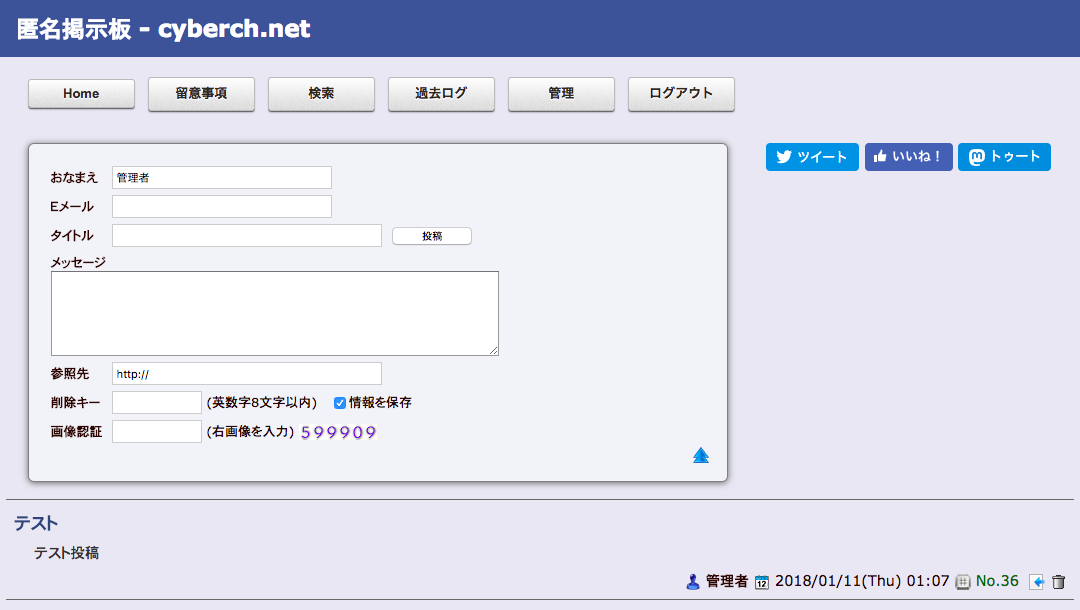
\includegraphics[width=130mm]{figures/bbs_screenshot.png}
	\end{center}
	\caption{匿名掲示板サイト}
	\label{fig: bbs_screenshot}
\end{figure}

掲示板への書込みの際に入力する項目は複数あるが,必須項目は書込みを行った人の名前,書込みのタイトル,本文,画像認証の4項目である.画像認証の項目には,入力欄の右側に画像として表示された数字を入力する.これはスパム投稿を防止するためのものである.先述の通り,名前は実名を入力する必要はないため,個人情報を一切入力せずに投稿できるため,利用者から見ると匿名掲示板のように利用することができる.必須項目を入力して投稿ボタンを押下すると投稿内容がサーバに送信され,書込み一覧に投稿内容が表示される.

\subsection{シェアボタンの設置}
LIGHT BOARDにはシェアボタンは設置されていない.本研究では,SNSのシェアボタンを利用して実験を行うため,シェアボタンを設置した.設置したSNSのシェアボタンは,Twitter,Facebook,Mastodonの3種類である.

Mastodonのシステムは,匿名掲示板サイトと同様に,本研究の実験用に用意したサーバ上に置かれている.そのため,Mastodonのシェアボタンを読み込む際に送信されたCookieは,保存,解析することができる.送信されたCookieを保存し,そのCookieからMastodonのユーザを特定するプログラムを作成した.詳細は後述する.

\subsection{同一ユーザ特定機能の実装}
LIGHT BOARDは,書込み時に名前の入力が必須であるが,同一ユーザが複数の書込みを行う際に,それぞれ異なる名前をつけることが可能である.そのため,複数の書込みが同一人物によるものかどうかを判断することは難しい.そこで,本研究の実験で使用する匿名掲示板には,ユーザを追跡するためのCookieを付与する機能を実装した.

初めて匿名掲示板にアクセスしてきたユーザには,サーバ側で生成したランダムな文字列をCookieとして付与する.2回目以降にアクセスしてきたユーザ(ブラウザ)は,初めてアクセスした際に付与されたCookieをサーバに送信するため,以前にアクセスしたことがあることがサーバ側でわかる.したがって,複数の書込みを行ったユーザは,書込みを行う際に送信しているCookieが同じであるため,同一人物による書込みであることがわかる.

ユーザを追跡するためのCookieを付与する機能に該当する箇所をソースコード\ref{track}に示す.

\begin{lstlisting}[caption=同一ユーザ特定機能,label=track]
use String::Random;

sub track {
  my $host = $ENV{REMOTE_HOST};
  my $addr = $ENV{REMOTE_ADDR};
  my $time = time;
  my ($min,$hour,$mday,$mon,$year,$wday) = (localtime($time))[1..6];
  my @wk = ('Sun','Mon','Tue','Wed','Thu','Fri','Sat');
  my $date = sprintf("%04d/%02d/%02d(%s) %02d:%02d",
        $year+1900,$mon+1,$mday,$wk[$wday],$hour,$min);
  my $cookie = $ENV{HTTP_COOKIE};

  my %cookie;
  foreach (split(/;/, $cookie)) {
    my ($key, $val) = split(/=/);
    $key =~ s/\s//g;
    $cookie{$key} = $val;
  }

  # もしトラッキング用のクッキーがセットされていればファイルに保存する
  # 保存されていなければ新しく発行してセットさせる
  if ($cookie{tracking_id}) {
    open(DAT, ">> $cf{trackingfile}") or error("open err: $cf{trackingfile}");
    my $new = "$date<>$cookie{tracking_id}<>$host<>$addr";
    print DAT "$new\n";
    close(DAT);
  }
  else {
    my $random = String::Random->new();
    my $tracking_id = $random->randregex("[a-zA-Z0-9]{64}");
    print "Set-Cookie: $cf{tracking_id}=$tracking_id\n";
  }
}
\end{lstlisting}

サブルーチンtrackは,トラッキング(特定)用のCookieが送信されなければ新たにCookieを発行し,送信されていればそのCookieをファイルに保存する.発行するCookieは,String::Randomを使用して生成した乱数を値とする.String::Randomを使用して生成する乱数は,大文字,小文字を区別した64文字の英数字であるため,他のユーザと重複する可能性は極めて低いと考えられる.よって,匿名掲示板への書込みとトラッキング用のCookieを照らし合わせ,複数の書込みに対して同じCookieが送信されている場合,同一人物による書込みであると判断できる.

\section{SNS}\label{sec: sns}
本研究では,SNSのアカウントを特定する実験を行うためのシステムとして,Mastodonを利用した.本来のサイバー犯罪においては,TwitterやFacebookなどの,世界的に利用されているSNSの運営と協力して犯人のアカウントを特定することを想定しているが,本研究の実験では,TwitterやFacebookのサーバ内の情報を閲覧することはできない.そこで,個人で運営することができる,Twitterに似たSNSであるMastodonを利用することで,シェアボタンを読み込む際に送信されるCookieからMastodonのアカウントを特定する実験を行った.送信されるCookieからアカウントを特定することは,TwitterやFacebookにおいても技術的に可能であるため,実際のサイバー犯罪ではTwitterやFacebookなどの運営と協力することで,犯人のアカウントが特定できるといえる.

\subsection*{Mastodon}
Mastodonとは,ドイツ人のEugen Rochko氏が,2016年2月に開発を開始した,分散型SNSのことである.Twitterに似た機能を持つSNSとして日本でも注目を集めている.オープンソースソフトウェアとしてGitHub上に公開されており,誰でも自由にプログラムを利用することができる.

TwitterやFacebookとは異なり,Mastodonはプログラムを改変することができ,また改変したプログラムをサーバ上に置いて運営することもできる.Mastodonは分散型SNSであり,個人や団体,企業などが運営するため,複数のサーバが存在する.Mastodonが運営されている各々のサーバのことを,Mastodonのインスタンスと呼ぶ.GitHubからダウンロードしたMastodonのプログラムに,本研究の実験に必要な機能を実装して利用した.

\subsection{シェアボタンの実装}
匿名掲示板に設置するシェアボタンの実装を行った./buttonというURLにアクセスすると,Mastodonのシェアボタンの画像だけが表示されるページを作成した.匿名掲示板では,HTMLのiframeタグを利用し,Mastodonのシェアボタンのページを読み込んでいる.

ユーザ(ブラウザ)は,匿名掲示板にアクセスした際に,Mastodonのシェアボタンを読み込むためにMastodonのサーバにアクセスする.Mastodonのサーバにアクセスする際に,もしユーザがMastodonにログインしている状態であれば,そのログイン状態を保持するCookieをMastodonのサーバに送信するため,匿名掲示板にアクセスしたユーザとMastodonにログインしているユーザを結びつけることができる.

\subsection{送信されたCookieを保存する機能の実装}\label{sec: save_cookie}
匿名掲示板に設置されたシェアボタンを通してMastodonのサーバに送信されたCookieをデータベースに保存する機能を実装した.Mastodonのシェアボタンが読み込まれた際に,送信元の情報を取得し,データベースに保存している.保存する送信元の情報を表\ref{tb: buttons_database}に示す.

\begin{table}[H]
	\caption{保存した送信元のデータ}
	\label{tb: buttons_database}
	\begin{center}
		\begin{tabular}{ | c | c | p{8cm} | } \hline
			データ & データ型 & データ例 \\ \hline
			IPアドレス & string & 133.19.169.6 \\ \hline
			Cookie & text & remember\_user\_token=ABCD1234; \_session\_id=EFGH5678; \_mastodon\_session=IJKL9012  \\ \hline
			リファラ & string & https://www.google.co.jp/ \\ \hline
			ユーザエージェント & string &  Mozilla/5.0 (Macintosh; Intel Mac OS X 10\_12\_6) AppleWebKit/537.36 (KHTML, like Gecko) Chrome/62.0.3202.94 Safari/537.36 \\ \hline
		\end{tabular}
	\end{center}
\end{table}

取得したデータは,IPアドレス,Cookie,リファラ,ユーザエージェントの4つである.データ型は,データベースに保存する際の型を意味する.データ例は,実際に保存されるデータの例を示している.

データベースには,Cookieの他に送信元のIPアドレスやリファラ,ユーザエージェントを保存している.本研究においてはCookieのみの保存で十分であるが,Cookieが取得できなかった場合や,より詳細な情報を得るために,Cookie以外の情報も保存することにした.

\subsection*{リファラ}
リファラとは,どのページからアクセスしたかを示す情報である.例えば,Googleの検索結果からリンクをクリックしてサイトAにアクセスした場合,ブラウザがサイトAに対して送信するリファラはhttps://www.google.co.jp/である.リンクをクリックしてページを遷移した場合に限らず,iframeを使用して別のサイトを読み込んだ場合にもリファラは送信される.匿名掲示板のHTML内に含まれるiframeタグからMastodonのページを読み込んだ場合,Mastodonのサーバに送信されるリファラは,匿名掲示板のURLである.このように,リファラはどのページを経由してアクセスしてきたかがサーバ側にわかるため,Webサイトの解析ツールなどでしばしば用いられる.

\subsection*{ユーザエージェント}
ユーザエージェントとは,ブラウザがサーバに対して送信する情報であり,使用しているブラウザやOS,またその種類などの情報が含まれている.例えば表\ref{tb: buttons_database}のデータ例の場合,アクセスしてきたユーザは,macOS 10.12.6を使用しており,Google Chrome 62.0.3202.94でアクセスしていることがわかる.使用しているブラウザごとにWebページの表示を変えるなど,ユーザビリティの向上を目的に使用されることもあるが,サイバー犯罪においては,犯人の使用しているOSやブラウザがわかるといった利点がある.ただし,ユーザエージェントは詐称(本来とは異なる情報をサーバ側に送信)することも可能であるため,必ずしもユーザエージェントと同じOSやブラウザを使用しているとは限らない.

\subsection{ブラウザフィンガープリンティングの実装}
Cookieやリファラ,ユーザエージェントなどはブラウザからサーバに送信される情報であるが,JavaScriptを使用することで,通常はサーバに送信されない情報を取得することができる.

JavaScriptはブラウザ上で実行されるスクリプト言語であり,Webページの遷移を行うことなくHTMLの構成要素を書き換えたり,非同期でサーバと通信したりすることができる.近年ではほとんどのWebサイトにJavaScriptが使用されている.また,JavaScriptを使用して,ブラウザやデバイスの情報を取得することができる.このように,Cookieの代わりにJavaScriptを利用して,ユーザが使用するデバイスを調べて同一ユーザを特定する仕組みをブラウザフィンガープリンティングという.

ブラウザフィンガープリンティングには,\ref{sec: save_cookie}項で説明したリファラやユーザエージェントなども含まれる.本研究の実験では,通常はサーバに送信されない情報である画面サイズを,JavaScriptを使用して取得することにした.JavaScriptを使用しないと取得できない情報を収集することで,より精度の高い特定手法を提案できると考えられるためである.

サーバ側で,ブラウザから送信された画面サイズの情報を受け取るためのAPIエンドポイントを作成した.APIエンドポイントとは,APIにアクセスする際のURLのことである.本研究では,/api/v1/fingerprintというエンドポイントを作成し,このエンドポイントに対してHTTPのPOSTリクエストが送信された場合に,送信された情報をデータベースに保存する機能を実装した.

JavaScriptでは,ユーザが使用するデバイスの画面サイズを取得し,サーバに送信するプログラムを実装した.該当するJavaScriptのプログラムをソースコード\ref{prog: fingerprint_js}に示す.

\begin{lstlisting}[caption=画面サイズの取得とサーバへの送信,label=prog: fingerprint_js]
var xhr = new XMLHttpRequest();
xhr.open('POST', '/api/v1/fingerprint', true);
xhr.setRequestHeader('content-type', 'application/x-www-form-urlencoded');
xhr.send('screen_size=' + screen.width + 'x' + screen.height);
\end{lstlisting}

JavaScriptでサーバにリクエストを送信する際には,XMLHttpRequest()を使用する.新しく生成したXMLHttpRequest()のオブジェクトを変数xhrに格納する.xhr.open()を使用して,HTTPメソッド(GETやPOSTなど)やリクエストを送信するURL(エンドポイント)を指定する.必要であればxhr.setRequestHeader()を使用してリクエストヘッダを設定することもできる.最後にxhr.send()を使用して,サーバに送信するデータを指定し,送信する.JavaScriptでデバイスの画面サイズを取得するにはscreen.width(画面横幅)とscreen.height(画面縦幅)を使用する.例えばscreen.widthで取得した値が1440,screen.heightで取得した値が900であった場合,'screen\_size=1440x900'という文字列をサーバに送信する.この情報を受け取ったサーバは,データベースにこのデータを文字列として保存する.

\section{実験用ツール}
匿名掲示板とSNSの他に,本研究の実験に当たって必要となるツールの実装を行った.

\subsection{UNIXタイム変換ツール}\label{sec: unix_time_translation}
匿名掲示板サイトへの書込みは,ファイルに保存するように実装されている.投稿された書込みを保存したファイルの一部を以下に示す.

\begin{verbatim}
5<>2017/12/13(Wed) 18:01<>baz<><>piyo<>ううう<><>133.19.169.6<><>1513155668<>
4<>2017/12/13(Wed) 17:59<>bar<><>huga<>いいい<><>133.19.169.6<><>1513155569<>
3<>2017/12/13(Wed) 17:51<>foo<><>hoge<>あああ<><>133.19.169.6<><>1513155083<>
2<>2017/12/13(Wed) 17:51<>xxx<><>xxx<>test<><>133.19.169.6<><>1513155081<>
1<>2017/12/13(Wed) 17:50<>なまえ<><>無題<>テスト<><>133.19.169.6<><>1513155034<>
\end{verbatim}

投稿された各々の書込みは行ごとに保存されており,書込み内容に関する情報を,\verb|<>|で区切って管理されている.保存されている情報は,左から順に,書込み番号(最初の書込みを1とした連番),投稿時刻,名前,書込みのタイトル,書込みの本文,IPアドレス,UNIXタイムスタンプである.

本研究の実験では,匿名掲示板への書込み時刻とSNSのシェアボタンを読み込む際に送信されたCookieの保存時刻を照合して,書込みを行ったユーザのSNSのアカウントを特定している.書込み内容を管理するファイルには,書込み時刻が保存されているが,秒数までは記録されていない.実際に実験を行ったところ,秒単位でのアクセスが集中したため,書込み時刻からは,Cookieの保存時刻と照合することができなかった.そこで,書込み時刻の代わりにUNIXタイムスタンプを確認することで,Cookieの保存時刻との照合を行った.本研究では,UNIXタイムスタンプを,秒数を含めた時刻に変換するプログラムをPerlで実装した.そのプログラムをソースコード\ref{prog: unix_to_localtime}に示す.

\begin{lstlisting}[caption=UNIXタイムスタンプ変換プログラム,label=prog: unix_to_localtime]
print "localtime: ";
my $num = <STDIN>;
my $time = $num;
my ($sec,$min,$hour,$mday,$mon,$year) = (localtime($time))[0..5];
my $date = sprintf("%04d-%02d-%02d %02d:%02d:%02d",$year+1900,$mon+1,$mday,$hour,$min,$sec);
print "timestamp: " . $date . "\n"
\end{lstlisting}

標準入力からUNIXタイムスタンプを受け取り,時刻に変換して出力するプログラムである.localtime関数は引数として受け取ったUNIXタイムスタンプを9つの要素の配列に変換する関数である\cite{localtime}.ソースコード\ref{prog: unix_to_localtime}では,localtime関数を使用して,入力されたUNIXタイムスタンプから,秒,分,時,日,月,年を取得し,それぞれ変数に格納している.sprintf関数を使用して表示する時刻のフォーマットを指定した後,標準出力を行っている.

\subsection*{UNIXタイムスタンプ}
UNIXタイムスタンプとは,1970年1月1日0時0分0秒を0として,その時刻からの経過秒数を数値で表したものである.たとえば,UNIXタイムスタンプが1513155034であった場合,1970年1月1日0時0分0秒からカウントして1513155034秒が経過した時点での時刻(2017年12月13日17時50分34秒)を表す.ファイルに保存された書込み時刻には秒数が記録されていないが,UNIXタイムスタンプから時刻に変換することで,書き込みがあった時刻の秒数を求めることができる.

\subsection{Railsセッションデコーダ}\label{sec: rails_session_decoder}
本研究の実験に使用するSNSであるMastodonは,Ruby on Rails(以下,Rails)と呼ばれるWebアプリケーションフレームワークを用いて実装されている.Webアプリケーションフレームワークとは,Webアプリケーションにおける一般的な機能を提供する雛形のことである.一般的なWebアプリケーションでは,Webサイトのフォームから入力された情報をデータベースに保存したり,データベースから取得した内容を表示したり,データベースに存在するデータを更新・削除したりする機能がある.それらの機能を,Webアプリケーションの開発者が1から実装することは,開発コストがかかるだけでなく,セキュリティに十分な注意を払わなければ脆弱性を生み出す危険性がある.Webアプリケーションフレームワークを利用すれば,少ない開発コストで,それらの機能を持ったWebアプリケーションを構築することができる.また,多くのWebアプリケーションフレームワークは,オープンソースソフトウェアとしてインターネット上に公開されているため,Webの脆弱性に対する対策が行われている.

ブラウザがWebサービスにログインしている情報は,通常,Cookieに保存されている.ログインに成立すると,サーバはブラウザに,ログイン状態を保持するセッション情報をCookieとして保存するように指示する.以降,セッション情報が含まれるCookieをブラウザがサーバに送信することで,サーバは,アクセスしてきたユーザがログイン済みであると認識する.

したがって,SNSのシステムにおいて,ブラウザから送信されたCookieを調べることで,そのCookieを送信してきたユーザのSNSのアカウントを特定することができる.\ref{sec: sns}節で述べたように,本研究で使用するMastodonに送信されたCookieはデータベースに保存される.ところが,Rails 4.0以降では,セッション情報が暗号化されてCookieに保存されている\cite{rails_session_is_encrypted}ため,そのままではMastodonのアカウントを特定することができない.そこで,データベースに保存されたCookieの中に含まれるセッション情報を複合するプログラムをNode.jsで実装した.そのプログラムをソースコード\ref{prog: rails_session_decoder}に示す.

\begin{lstlisting}[caption=Railsセッションデコーダ,label=prog: rails_session_decoder]
const rsd = require('rails-session-decoder');
const read = require('readline-sync');
const fs = require('fs');

var cookie = read.question('Input your cookie: ');
var key = read.question('Input your secret key: ');

console.log('');

var decoder = rsd(key);

decoder.decodeCookie(cookie, (err, data) => {
  if (data) {
    console.log(data);
  }
  else {
    console.log(err);
  }
});
\end{lstlisting}

暗号化されたセッション情報を復号するには,セッション情報を含むCookieとRails(Mastodon)システム内で管理されている秘密鍵が必要である.セッション情報を含むCookieはデータベースに保存されているものを使用し,秘密鍵はRails(Mastodon)の設定ファイルに書かれているものを使用する.

ソースコード\ref{prog: rails_session_decoder}は,標準入力から,暗号化されたセッション情報を含むCookieと,秘密鍵を受け取り,暗号化されたセッション情報の復号を行う.正しく復号できた場合は復号されたセッション情報を出力し,正しく復号できなかった場合はエラーを出力する.

暗号化されたセッション情報の復号には,rails-session-decoderというNode.jsのパッケージ(ライブラリ)を利用した\cite{npm_rails_session_decoder}.rails-session-decoderを読み取ったオブジェクトに対して,暗号化されたセッション情報を含むCookieと秘密鍵を渡してdecodeCookieメソッドを呼び出すと,暗号化されたセッション情報が復号される.ユーザ(ブラウザ)から送信されたCookieがセッション情報を含んでいれば,復号に成功する.






\chapter{実験}
\section{実験手順}
本研究では,SNSのシェアボタンを読み込む際に送信されるCookieから,SNSのアカウントを特定する実験を行った.本実験の目的は,Webサイトに設置されているSNSシェアボタンを利用した,SNSのアカウントの特定可能性を検証するためである.本実験では,TwitterやFacebookに代わるSNSとして,Mastodonを利用した.

本実験を被験者として,立命館大学情報理工学部サイバーセキュリティ研究室に所属する学部生15名に協力してもらった.被験者15名には,本研究で用意した匿名掲示板とSNSサイトに対して,以下の事柄を実行してもらった.

\begin{enumerate}
\item{Mastodonアカウントの作成}
\item{メールアドレスの確認とMastodonへのログイン}
\item{匿名掲示板へのアクセス}
\item{匿名掲示板への書込み}
\end{enumerate}

\subsection{Mastodonアカウントの作成}
通常,Mastodonのインスタンスをインターネット上に公開した場合,誰でもそのインスタンスにアカウントを作成することができる.ただし,Mastodon v2.1.0以降では,招待システムが導入され,招待用のリンクを知っている者のみがアカウントを登録することができる\cite{invite_system}.外部の第三者(本実験の被験者ではない者)が,本研究で用意したMastodonインスタンスにアカウントを登録できる状態になっていた場合,本実験で得られるデータの収集の妨げになると判断したため,本研究のMastodonインスタンスでは,招待リンクを知っている者のみがアカウントを登録できるように設定した.事前に招待用のリンクを被験者に配布した.

匿名掲示板へ書込みを行った被験者のMastodonアカウントを特定するため,被験者にはMastodonのアカウントを作成してもらった.アカウント登録ページを図\ref{fig: account_registration}に示す.

\begin{figure}[H]
	\begin{center}
		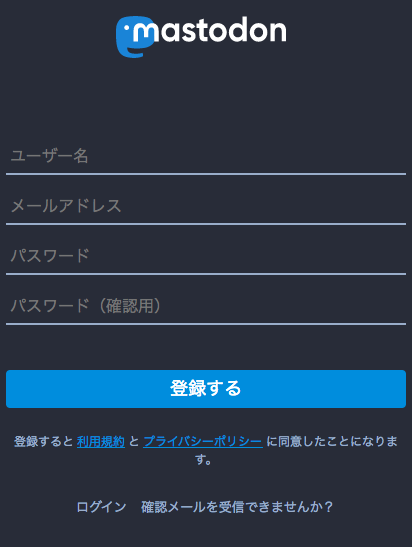
\includegraphics[width=130mm]{figures/account_registration_screenshot.png}
	\end{center}
	\caption{Mastodonアカウント登録ページ}
	\label{fig: account_registration}
\end{figure}

一般的なWebサービスのアカウント登録ページである.被験者は,このフォームにユーザー名(任意の文字列),メールアドレス,パスワードを入力して,アカウントを作成する.

\subsection{メールアドレスの確認とMastodonへのログイン}
アカウントを登録すると,登録時に入力したメールアドレス宛に確認メールが届く.届いたメールに記載されているリンク先にアクセスするとメールアドレスが確認される.登録したアカウントのメールアドレスの有効性が確認できるまで(確認メールのリンク先にアクセスするまで)は,アカウントにログインすることができない.

被験者は,メールアドレスの確認を行った後,ログインページにアクセスしてログインする.

\subsection{匿名掲示板へのアクセス}
被験者は,Mastodonにログインした状態で,匿名掲示板にアクセスする.匿名掲示板もMastodonと同様に,外部から利用されることを防ぐため,アクセス用のパスワードを設置した.アクセス用のパスワードは被験者のみに共有し,第三者から勝手に書込みが行われないようにした.パスワードを入力すると,\ref{sec: bbs}節で示した図\ref{fig: bbs_screenshot}のページが表示される.なお,図\ref{fig: bbs_screenshot}のページにはSNS(Mastodon)のシェアボタンが設置されているため,Mastodonのアカウントにログインした状態でこのページにアクセスした時点で,Mastodonインスタンスにログイン状態を保持するCookieが送信されている.

\subsection{匿名掲示板への書込み}
最後に,被験者は,図\ref{fig: bbs_screenshot}のページから適当な書込みを行う.書き込む際の名前や書込み内容などは,各々の被験者に一任した.また,同一人物が異なる名前で複数の書込みを行っても同一人物による書込みを特定できることを証明するために,一部の被験者には異なる名前で複数の書込みを行ってもらった.

\subsection{匿名掲示板への投稿時の注意点}
匿名掲示板への投稿時に以下の事柄に注意して投稿するよう被験者に説明した.

\begin{itemize}
\item{Mastodonアカウントにログインした状態で投稿すること}
\item{ログインした端末・ブラウザで投稿すること}
\end{itemize}

Mastodonアカウントにログインした状態で書込みを行わなければ,ログイン状態を保持するCookieが送信されないため,アカウントを特定することができない.そのため,被験者には,Mastodonアカウントを作成するだけでなく,作成したアカウントにログインした状態で書込みをするよう指示した.

また,Mastodonアカウントにログインした状態であっても,ログインしたものとは異なる端末・ブラウザを使用して書込みを行った場合も同様に,ログイン状態を保持するCookieが送信されない.そのため,ログインしたものと同じ端末・ブラウザを使用するよう指示した.また,ログインしたものと同じブラウザを使用したとしても,ブラウザのシークレットモード(プライベートブラウジングモード)を使用して書込みを行わないよう指示した.シークレットモードでは,閲覧履歴やCookieがリセットされた状態でブラウジングを行うようになるためである.ただし,シークレットモードでもう一度アカウントにログインし直した場合はこの限りではない.

\section{実験内容}\label{sec: exp_flow}
% 実験結果の前に,アカウントを特定するまでの流れを書こう.データベースからCookieを引っ張り出してきて,セッションデコーダにかけて復号して,得られたユーザIDからアカウント名を特定する流れ.
匿名掲示板に投稿された書込みすべてに対して,書込みを行ったユーザのMastodonのアカウントを特定した.アカウントを特定するまでの手順を以下に示す.

\begin{enumerate}
\item{書込みとCookieの紐付け}
\item{Cookieに含まれるセッション情報の復号}
\item{アカウント名の検索}
\end{enumerate}

\subsection{書込みとCookieの紐付け}
\ref{sec: unix_time_translation}項で示したように,匿名掲示板に投稿された書込みの書込み時刻をUNIXタイムスタンプから算出する.書込みが投稿された直後にSNSのシェアボタンが読み込まれCookieが送信されるはずである.したがって,書込みの直後に送信されたCookieを調べればよい.

匿名掲示板へ書き込まれた時刻が2017年12月13日17時51分21秒であったとする.その直後に送信されたCookieをMastodonのデータベースから検索する.その際に実行したSQLをソースコード\ref{prog: post_search_sql}に示す.

\begin{lstlisting}[caption=2017年12月13日17時50分34秒にあった書込みに対応するCookieを検索するSQL,label=prog: post_search_sql]
SELECT * FROM buttons WHERE created_at BETWEEN '2017-12-13 08:51:00' AND '2017-12-13 08:52:00' ORDER BY created_at;
\end{lstlisting}

挿入された日時が,2017年12月13日17時51分00秒から2017年12月13日17時52分00秒までの期間であるレコードを,buttonsテーブルから検索し,挿入された日時順に並び替えて表示するSQLである.ただし,Mastodonで使用するデータベースでは,時刻が日本標準時ではなくグリニッジ標準時として保存されてしまっていたため,実際の時刻より9時間前の時刻で検索している.

buttonsテーブルには,Mastodonのシェアボタンを読み込み際に送信されたCookieが保存されている.保存されているデータは表\ref{tb: buttons_database}の通りである.Railsで扱うデータベースには,すべてのテーブルにレコードの作成日時と更新日時が自動で追加される.ソースコード\ref{prog: post_search_sql}で使用しているcreated\_atはレコードの作成日時に該当する.検索結果は,指定した期間内のレコードの作成日時順に,該当するレコードを表示している.つまり,書込みがあった時刻に近い範囲の時刻で送信されているCookieをすべて表示するSQLとなっている.

表示された複数のレコードのうち,書込み時刻よりも後であり,最も書込み時刻に近いレコードを調べる.そのレコードに保存されているIPアドレスやユーザエージェントが,書込みのものと一致していれば,そのレコードが書込みに対応するものであると判断する.なお,匿名掲示板側のIPアドレスは匿名掲示板への書込みが保存されたファイル内に保存されているもの,ユーザエージェントはWebサーバのログに保存されているものを利用した.
% リファラで本当に送信元が匿名掲示板なのかをチェックしたってことも書く?
% フィンガープリンティングの情報も念押しのためにチェックしたことも書く?

\subsection{Cookieに含まれるセッション情報の復号}
書込み情報と一致したレコードからCookieを調べる.例として,2017年12月13日17時51分21秒に投稿された書込みと一致するレコードのCookieは以下の通りである.

\begin{verbatim}
_mastodon_session=TzhBbE5SWVBjcXBmakgzQlZFclpqRExDMFB3WXJiSFdk
emQ4VkI3TThaNUlENmJGeGpOOVR4azJSVVVZUFVjQVlKL1pack1VTzRNdkpvcF
h4c2o1czFPVkliR3dpdHJpZ3Azb0VneEhZUVp2d1ZEbDE0MnJEZ2srbEk1L2ZJ
Q2ZPc1ZWU09DL0VDcVJhNG15aTZmWTZQMDhDc2pKS2VUdWdITmR1TWFqRGZOdW
hoc0gxeFhaYU5GWTlMY1BvZ29uK1V2RE1KSnFaU2Vvb28wS2dFVHBDS3ZXRWhR
S0FaVlhZQnM2NUJ4ZjNkTEdaNUVFek9pWGxyaUtZN01kWDBFTzBxa1FjTkdXU2
5IaklqVlUzeUs2MGVjV1hoNm8xdHFWWkxWcnhjeDU1UDdJNXVkZEpiNUVUUmJT
ekdTSkljaDhyT2dGM092ZVprbGcrS0pLR0JUZjg1dlpSNG0zNmRDY2lHVnB2WT
hYMy9ScC8rWk8zWjBIenZ3bmJJTGJhRDRRbnJpQUtlQXNTRHFDTDNQQjUyVmF6
UT09LS1JTG00Wlc4b0g5Vk9rZWJwUlpqUTlBPT0%3D--7c1f476c80f45229f4
f5b5f18d260e266f8f5930; _session_id=IjA5ZGMxYmQ5ZDIzOTFlNzJjMz
dlNDFmYzhlMGUyNWQxIg%3D%3D--f749083440458553e2dfe0b45f1a226e6d
5407e5; remember_user_token=W1szXSwiJDJhJDEwJDBtekVCUXo0cFR4bT
hCNVI5dDFhT2UiLCIxNTEzMTU0NzkwLjgxMDU4MTciXQ%3D%3D--0e2f0c3b4c
71e16a9828e0d0424cfe7545ba92df
\end{verbatim}

Cookieは,名前と値のペアをイコール記号で結んだ形式となっている.左辺が名前で,右辺が値である.複数のペアを一つのCookieにまとめる場合はセミコロンで区切る.

上記Cookieは,\verb|_mastodon_session|と\verb|_session_id|と\verb|remember_user_token|の3つで構成されている.ログイン状態のユーザ(ブラウザ)がMastodonに送信するCookieはこの3つの名前を持つ値であり,このうち,ログイン状態を保持するセッション情報を持つCookieは\verb|_mastodon_session|である.

\verb|_mastodon_session|を,\ref{sec: rails_session_decoder}項で説明したRailsセッションデコーダを使用して復号すると,以下の情報が得られる.

\begin{verbatim}
{
  "session_id":"fb177bece158591f43126c67987159f1",
  "warden.user.user.key":[[3],"$2a$10$0mzEBQz4pTxm8B5R9t1aOe"],
  "user_return_to":"/button?text=%e6%8e%b2%e7%a4%ba%e6%9d%bf%e3
  %81%8b%e3%82%89%e3%81%93%e3%82%93%e3%81%ab%e3%81%a1%e3%81%af%
  ef%bc%81",
  "_csrf_token":"WgC1EbiMg3YV1VgqJNwCNkgw6ldgRwS1Qkz3ckUm/SM="
}
\end{verbatim}

得られた情報が,Mastodonのシェアボタンを読み込む際に送信されたCookieから復号されたセッション情報である.このセッション情報のうち,\verb|warden.user.user.key|の中の3という数値が,Cookieを送信してきたユーザのユーザIDである.

\subsection{アカウント名の検索}
得られたユーザIDをもとにMastodonのデータベースで検索を行う.ユーザIDが3であるユーザを検索するSQLをソースコード\ref{prog: user_search_sql}に示す.

\begin{lstlisting}[caption=ユーザIDが3であるユーザを検索するSQL,label=prog: user_search_sql]
SELECT * FROM users WHERE id = 3;
\end{lstlisting}

ユーザに関する情報はusersテーブルに保存されている.ここには,アカウント登録時に入力したメールアドレスや暗号化されたパスワードなどのユーザ情報が保存されている.さらに,メールアドレスや暗号化されたパスワードとともにアカウントIDが保存されている.ユーザIDが3であるユーザのアカウントIDは3であることがわかった.この結果をもとにアカウントIDが3であるアカウントを検索するSQLをソースコード\ref{prog: account_search_sql}に示す.

\begin{lstlisting}[caption=アカウントIDが3であるアカウントを検索するSQL,label=prog: account_search_sql]
SELECT * FROM accounts WHERE id = 3;
\end{lstlisting}

アカウントに関する情報はaccountsテーブルに保存されている.accountsテーブルには,アカウント登録時のユーザ名が保存されている.\ref{sec: exp_flow}に示す一連の作業を実行すると,結果として,匿名掲示板に書込みを投稿した者のMastodonのユーザ名を特定することができる.ユーザ名を特定することで,そのアカウントに登録されているメールアドレスなどを特定することができる.実際のサイバー犯罪でこの手法を活用する場合,犯人のTwitterやFacebookなどのアカウントを特定することで,本実験以上に犯人を特定する情報が得られることが期待できる.

\section{実験結果}\label{sec: exp_result}
本実験の被験者15名に本実験に協力してもらったところ,計32件(自身による実験概要の説明のための書込みを除く)の書込みがあった.32件の書込みすべてに対して,\ref{sec: exp_flow}節で説明した手順を実行してアカウントの特定を行った.その結果を表\ref{tb: exp_result}に示す.


% データに間違いがないことの最終確認を行う!!
\begin{table}[H]
	\caption{実験結果}
	\label{tb: exp_result}
	\begin{center}
		\scalebox{0.85} {
			\begin{tabular}{ | c | c | c | c | c | c | c | } \hline

番号 & IPアドレス & Cookie ID & アカウントID & ユーザ名 & 書込み時刻 & Cookie送信時刻 \\ \hline
2 & (学外) & 33 & (特定不可) & \shortstack{ユーザα\\(特定不可)} & 2017-12-13 17:50:34 & 2017-12-13 17:50:37 \\ \hline
3 & 133.19.169.6 & 35 & 3 & ユーザA & 2017-12-13 17:51:21 & 2017-12-13 17:51:23 \\ \hline
4 & 133.19.169.6 & 37 & 7 & ユーザB & 2017-12-13 17:51:23 & 2017-12-13 17:51:29 \\ \hline
5 & 133.19.169.6 & 49 & (特定不可) & \shortstack{ユーザβ\\(特定不可)} & 2017-12-13 17:59:29 & 2017-12-13 17:59:36 \\ \hline
6 & 133.19.169.6 & 55 & 4 & ユーザC & 2017-12-13 18:01:08 & 2017-12-13 18:01:11 \\ \hline
7 & (学外) & 57 & 2 & ユーザD & 2017-12-13 18:01:23 & 2017-12-13 18:01:26 \\ \hline
8 & 133.19.169.6 & 59 & 10 & ユーザE & 2017-12-13 18:01:27 & 2017-12-13 18:01:30 \\ \hline
9 & (学外) & 62 & 15 & ユーザF & 2017-12-13 18:01:35 & 2017-12-13 18:01:41 \\ \hline
10 & 133.19.169.6 & 64 & 12 & ユーザG & 2017-12-13 18:01:46 & 2017-12-13 18:01:49 \\ \hline
11 & 133.19.169.6 & 75 & 16 & ユーザH & 2017-12-13 18:02:44 & 2017-12-13 18:02:46 \\ \hline
12 & (学外) & 77 & 13 & ユーザI & 2017-12-13 18:03:01 & 2017-12-13 18:03:04 \\ \hline
13 & (学外) & 78 & 9 & ユーザJ & 2017-12-13 18:03:10 & 2017-12-13 18:03:14 \\ \hline
14 & (学外) & 81 & 8 & ユーザK & 2017-12-13 18:03:15 & 2017-12-13 18:03:23 \\ \hline
15 & (学外) & 86 & 5 & ユーザL & 2017-12-13 18:03:31 & 2017-12-13 18:03:44 \\ \hline
16 & (学外) & 93 & 15 & ユーザF & 2017-12-13 18:04:06 & 2017-12-13 18:04:09 \\ \hline
17 & (学外) & 92 & 11 & ユーザM & 2017-12-13 18:04:06 & 2017-12-13 18:04:08 \\ \hline
18 & 133.19.169.6 & 104 & (特定不可) & \shortstack{ユーザβ\\(特定不可)} & 2017-12-13 18:04:24 & 2017-12-13 18:04:42 \\ \hline
19 & 133.19.169.6 & 100 & 4 & ユーザC & 2017-12-13 18:04:27 & 2017-12-13 18:04:29 \\ \hline
20 & 133.19.169.6 & 108 & 7 & ユーザB & 2017-12-13 18:05:11 & 2017-12-13 18:05:13 \\ \hline
21 & 133.19.169.6 & 109 & 3 & ユーザA & 2017-12-13 18:05:15 & 2017-12-13 18:05:17 \\ \hline
22 & 133.19.169.6 & 116 & 12 & ユーザG & 2017-12-13 18:05:29 & 2017-12-13 18:05:31 \\ \hline
23 & 133.19.169.6 & 120 & (特定不可) & \shortstack{ユーザβ\\(特定不可)} & 2017-12-13 18:05:33 & 2017-12-13 18:05:35 \\ \hline
24 & (学外) & 122 & 2 & ユーザD & 2017-12-13 18:05:44 & 2017-12-13 18:05:46 \\ \hline
25 & 133.19.169.6 & 132 & (特定不可) & \shortstack{ユーザα\\(特定不可)} & 2017-12-13 18:06:47 & 2017-12-13 18:06:49 \\ \hline
26 & (学外) & 134 & 9 & ユーザJ & 2017-12-13 18:07:01 & 2017-12-13 18:07:04 \\ \hline
27 & (学外) & 136 & 9 & ユーザJ & 2017-12-13 18:07:54 & 2017-12-13 18:07:56 \\ \hline
28 & 133.19.169.6 & 138 & (特定不可) & \shortstack{ユーザα\\(特定不可)} & 2017-12-13 18:08:14 & 2017-12-13 18:08:16 \\ \hline
29 & 133.19.169.6 & 144 & 12 & ユーザG & 2017-12-13 18:09:10 & 2017-12-13 18:09:12 \\ \hline
30 & 133.19.169.6 & 145 & 7 & ユーザB & 2017-12-13 18:09:11 & 2017-12-13 18:09:14 \\ \hline
31 & (学外) & 146 & 15 & ユーザF & 2017-12-13 18:09:22 & 2017-12-13 18:09:25 \\ \hline
32 & 133.19.169.6 & 169 & 7 & ユーザB & 2017-12-13 18:13:48 & 2017-12-13 18:13:50 \\ \hline
34 & (学外) & 214 & 12 & ユーザG & 2017-12-16 16:18:02 & 2017-12-16 16:18:05 \\ \hline

			\end{tabular}
		}
	\end{center}
\end{table}

% 連番になっていないことの説明をすること(自身の書込みのことを説明)
% ユーザ名は,具体的なものではなく,ユーザA,ユーザB,ユーザC,...とする.

表中の「番号」は匿名掲示板への書込み番号(連番),Cookie IDは送信されたCookieを管理するためのデータベース上のユニークな番号(連番),アカウントIDはアカウントを管理するためのデータベース上のユニークな番号(連番)を表す.番号1,33,35は,自身の実験概要の説明のための書込みであるため,省略している.書込み時刻は匿名掲示板への書込みが行われた時刻,Cookie送信時刻は匿名掲示板への書込みに対応するCookieが送信された時刻を表す.また,IPアドレスが133.19.169.6となっているものは立命館大学内のネットワークからのアクセスであり,それ以外のネットワークからアクセスされた際のIPアドレス(モバイル端末など)は(学外)とした.

32件中,26件の書込みは特定することができたが,残りの6件は特定することができなかった.その原因は,匿名掲示板への書込み後,SNSシェアボタンを読み込むアクセスはあったが,そのアクセスの際にCookieが送信されていなかったためである.特定できなかった6件の書込みの送信元情報を表\ref{tb: exp_result_untracked}に示す.なお,ユーザエージェントは長いため,それぞれ共通の部分は省略している.

\begin{table}[H]
	\caption{特定できなかった書込みの送信元情報}
	\label{tb: exp_result_untracked}
	\begin{center}
		\scalebox{0.85} {
			\begin{tabular}{ | c | c | c | c | } \hline

番号 & IPアドレス & ユーザエージェント & 画面サイズ \\ \hline
2 & (学外) & Windows NT 10.0; WOW64 Vivaldi/1.91.867.38 & 1280x720 \\ \hline
5 & 133.19.169.6 & Windows NT 6.3; Win64; x64 Chrome/63.0.3239.84 & 1280x720 \\ \hline
18 & 133.19.169.6 & Windows NT 6.3; Win64; x64 Chrome/63.0.3239.84 & 1280x720 \\ \hline
23 & 133.19.169.6 & Windows NT 6.3; Win64; x64 Chrome/63.0.3239.84 & 1280x720 \\ \hline
25 & 133.19.169.6 & Windows NT 10.0; WOW64 Vivaldi/1.91.867.38 & 1280x720 \\ \hline
28 & 133.19.169.6 & Windows NT 10.0; WOW64 Vivaldi/1.91.867.38 & 1280x720 \\ \hline

			\end{tabular}
		}
	\end{center}
\end{table}

本実験は,立命館大学内のネットワークを使用した被験者が多かったため,IPアドレスでの特定は困難である.また,特定できなかった書込みの送信元の画面サイズの情報は,6件すべて同じであった.ところが,ユーザエージェントが,番号2,25,28と,5,18,23とでそれぞれ全く同じであったため,特定できなかった6件の書込みは,2名の被験者によって書き込まれていることがわかった.これは,被験者15名に対して,特定できた被験者がユーザAからユーザMまでの13名であり,特定できなかった被験者が2名いることに符合する.ちなみに,番号2,25,28の書込みを行った被験者が,番号2では学外のネットワークからアクセスしているのに対し,番号25,28では学内のネットワークからアクセスしていることがわかる.

\subsection{実験結果の正答率}
実験を行い,実験結果をまとめた後,実験結果が正しいかどうかを確認した.具体的には,それぞれの書込みに対して,特定したアカウントが正しいかどうかを,被験者本人に確認した.また,特定できなかった書込みに対して,特定できなかった原因を調査した.

ユーザA,ユーザB,ユーザC,...(以降省略)がそれぞれ誰であるかを確認した.それぞれのユーザ(被験者)に対して,書込み番号に対応する書込みを行ったかどうかを確認した.その結果,特定できたすべての書込みに対して,特定したアカウント(被験者)が正しいことがわかった.

特定できなかった2名の被験者(表\ref{tb: exp_result}中のユーザαとユーザβ)に対しても同様に,書込み番号に対応する書込みを行ったかどうかを確認した.ユーザαの書込みとユーザβの書込みのうち,どちらの書込みを行ったかを2名の被験者それぞれに申告してもらい,ユーザα,ユーザβとして分類した書込みが,それぞれ同一人物による書込みであることを確認した.また,それぞれの被験者のユーザエージェントが正しいこと(ユーザエージェントから推測可能な,使用しているOS,ブラウザやそれらのバージョン)も確認した.












\chapter{評価と考察}
% 考察には,以下のことを書く.
% ほとんど学内のWi-Fiからだけど,特定できた
% 匿名掲示板に異なる名前で投稿していても,特定できた
% 同じユーザが別のネットワークから書き込んでも,特定できた
% 特定できなかったのは,ブラウザの機能や拡張機能によるものである

\section{考察}
% 特定できなかったのは,ブラウザの機能や拡張機能によるものである
\subsection{Cookieが送信されない原因に対する考察}
本実験では,被験者15名のうち,13名のアカウントを特定することができたが,残り2名を特定することができなかった.その原因は,\ref{sec: exp_result}節で述べた通り,Cookieが送信されていなかったためである.アカウントにログインしており,シェアボタンを読み込むアクセスがあるにもかかわらず,Cookieが送信されなかった要因について考察する.

\subsubsection{サードパーティCookieのブロック}
サードパーティCookieとは,デジタルマーケティングラボの記述を引用すると「ユーザーが訪問しているWebサイトのドメイン以外から発行されているCookieのこと」である\cite{what_is_third_party_cookie}.Cookieは,ブラウザがWebサーバのリソースにアクセスする際に送信されるが,閲覧するWebサイトとは異なるドメインのサーバに送信するCookieのことをサードパーティCookieと呼ぶ.閲覧するWebサイトのサーバに送信するCookieは,サードパーティCookieに対してファーストパーティCookieと呼ばれる.

本実験では,匿名掲示板サイトにSNSのシェアボタンが設置されているため,匿名掲示板にアクセスすると,ブラウザはSNSのシェアボタンを読み込むためにSNSのサイトにもアクセスすることになる.SNSのシェアボタンを読み込む際に,SNSのサイト用のCookieがSNSのサーバに送信されるが,ここで送信されているSNSのCookieは,本来アクセスしているWebサイト(匿名掲示板)とは異なるサイトのCookieであるため,サードパーティCookieである.

サードパーティCookieは,Webサイトに埋め込まれた広告などで使用され,ユーザの趣向に合った広告を表示するなど,ユーザビリティ向上の面で利用されることもある.一方で,サードパーティCookieは,どのようなWebサイトに送信されているかがユーザにとってわかりにくく,知らないうちにユーザの閲覧情報を収集されてしまう危険性があるため,プライバシー問題が懸念される\cite{third_party_cookie_is_danger}.

こうしたプライバシー問題の観点から,Webユーザは,サードパーティCookieをブロックする(送信しない)ことができる.最も簡単な方法は,ブラウザの設定を変更することである.近年のWebブラウザでは,サードパーティCookieをブロックする機能が実装されている.Google Chrome 63の場合,chrome://settings/content/cookiesにアクセスし,「サードパーティの Cookie をブロックする」という項目を有効にするとサードパーティCookieが送信されなくなる.

\begin{figure}[H]
	\begin{center}
		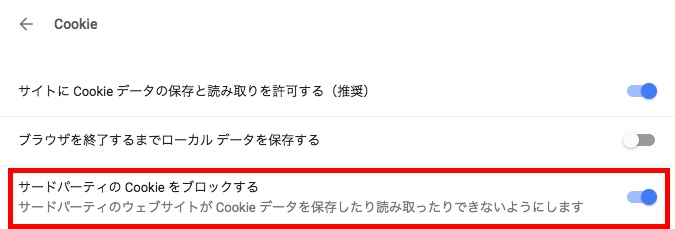
\includegraphics[width=130mm]{figures/disable_third_party_cookie_on_chrome.png}
	\end{center}
	\caption{Google ChromeにおけるサードパーティCookieのブロック}
	\label{fig: disable_third_party_cookie_on_chrome}
\end{figure}

\noindent
Firefox 57の場合,about:preferences\#privacyにアクセスし,履歴セクションの項目を「記憶させる履歴を詳細設定する」に変更し,「サードパーティ Cookie の保存」の項目を「常に拒否」に変更するとサードパーティCookieが送信されなくなる\cite{how_to_disable_third_party_cookie_on_firefox}.

\begin{figure}[H]
	\begin{center}
		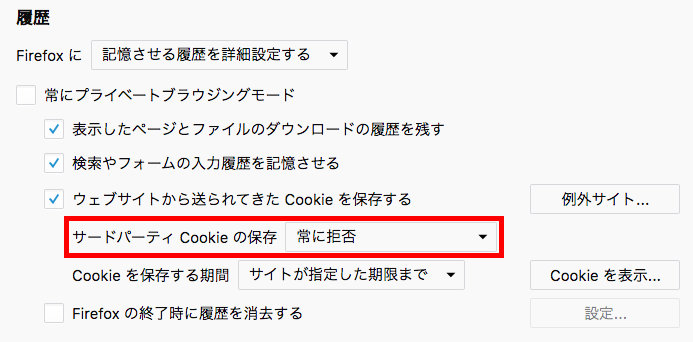
\includegraphics[width=130mm]{figures/disable_third_party_cookie_on_firefox.png}
	\end{center}
	\caption{FirefoxにおけるサードパーティCookieのブロック}
	\label{fig: disable_third_party_cookie_on_firefox}
\end{figure}

また,サードパーティCookieをブロックする拡張機能やアドオンも存在する.たとえば,Ghosteryはトラッキングツールや解析ツールをブロックする拡張機能として有名であり,Google ChromeやFirefoxのほか,ほとんどのモダンWebブラウザで利用可能である.Ghosteryをインストールしたブラウザで匿名掲示板にアクセスして,Mastodonインスタンスのデータベースを調べたところ,Cookieが送信されていないことがわかった.Ghosteryを無効にして再度確認するとサードパーティCookieが送信されたことから,GhosteryはサードパーティCookieのブロック機能が実装されていることがわかる.

このように,ユーザ側でサードパーティCookieをブロックしていると,本研究の手法ではSNSのアカウントを特定できないことがわかった.本実験おいて,アカウントを特定することができなかった被験者2名は,いずれもブラウザの設定でサードパーティCookieをブロックする機能を有効にしていた.Mastodonアカウントにログインした状態にもかかわらずCookieが送信されなかったのは,ブラウザによるサードパーティCookieのブロックが原因であると考えられる.

% 匿名掲示板に異なる名前で投稿していても,特定できた
% 同じユーザが別のネットワークから書き込んでも,特定できた
\subsection{異なる情報を送信した場合の特定可能性における考察}
IPアドレスによる特定の場合,様々なネットワークに切り替えて犯行に及ぶ犯人を特定するのは非常に困難である.一方で,Cookieの送信に関しては,ブラウザがサーバにアクセスする度に同意を求めるものではないため,ユーザがCookieの送信を意識することはあまり多くないと考えられる.また,過度なCookieのブロックは利便性を損なうため,ブラウジングにおいてすべてのCookieをブロックするユーザはほとんどいないと考えられる.

本研究では,Cookieの中でも,情報を収集されていることが気づきにくいとされるサードパーティCookieに着目し,実験を行った.実験の結果,サードパーティCookieがブロックされない限り,この手法におけるサイバー犯罪の犯人の特定可能性(本実験ではSNSアカウントの特定可能性)が十分に期待できると考えられる.本実験では,匿名掲示板に書き込む際の名前を変更したり,実験の途中で異なるネットワークに切り替えたりする被験者がいたが,その場合でもCookieから特定することが可能であった.サードパーティCookieの送信は気づきにくいため,実際のサイバー犯罪において,用心深い犯人であっても,不注意によりサードパーティCookieを送信する場合が考えられる.一度でもCookieの送信が確認されれば,犯人を特定できる可能性は十分あるといえる.

% ほとんど学内のWi-Fiからだけど,特定できた
\subsection{同一ネットワーク上の特定可能性における考察}
本実験は学内で行ったため,学内ネットワークを使用する被験者が比較的多かった.
%ネットワークは組織レベルだけど,Cookieはブラウザ・端末レベルだからより細かい追跡ができる的なことをメリット的な感じで書きたい.ほとんど学内のWi-Fiからのアクセスでも特定できたことを何かしらのメリットとして書く

\section{評価}






















\chapter{結論}
\section{まとめ}
% 最近のWebサイトではSNSシェアボタンを設置しているところも多いので役に立つんじゃなかろうか
近年のWebサイト,とりわけニュースサイトやブログサイトでは,閲覧者に記事を広めてもらうために,SNSシェアボタンを設置するケースが珍しくない.本実験により,SNSシェアボタンを読み込む際に送信されるCookieが個人を特定するのに十分な情報であることがわかったため,サイバー犯罪の犯人特定に有効であると考えられる.

% サードパーティCookieはCookieの中でも送信していることに気づきにくいため追跡する手法として有用である
Cookieはユーザを追跡する用途で使用されることもある.例として,以前にそのWebサイトにアクセスしたユーザであるかどうかを特定することができる.その中でも,サードパーティCookieはユーザがアクセスしているWebサイトとは異なるWebサイトに送信されるCookieであるため,ユーザが情報を収集されていることに気づきにくい.本実験では,15名の被験者のうち,13名のCookieを収集し,特定することができた.

% またサイバー犯罪の被害を受けたサーバに残った情報(ログなど)だけでなく外部のSNSと協力することでより特定率が大きくなるのではなかろうか
サイバー犯罪が発生した際に,Webサーバに残る情報だけでは犯人を特定することができない場合もある.サイバー犯罪の被害を受けたサーバに記録された情報(Webサーバのログなど)だけでなく,SNSの運営側と協力することで,犯人特定可能性がより大きくなるのではないかと考えられる.

% 今回の実験ではSNSとの協力を主軸に置いたがたとえば広告業者と協力することでも犯人特定できるんじゃないかな
本実験では,外部に起因する情報としてSNSシェアボタンを採用した.近年のWebサイトでは,SNSシェアボタンの他に,広告を設置しているものが多く見受けられる.外部の広告業者の広告を掲載している場合は,SNSシェアボタンと同様に,広告を運営するサービスのサーバにCookieが送信される.実際に,広告業者はユーザが興味のある広告を提供するためにCookieを使用している\cite{third_party_cookie_is_danger}.サイバー犯罪の犯人の特定においては,ユーザビリティ向上の目的で使用されている広告のCookieを解析することで,犯人に関する情報を収集することが可能であると考えられる.SNSシェアボタンの代わりに広告のCookieを利用することでも,本実験と同様の手法を実現することができるといえる.

% ところがサードパーティCookieを無効にすることも可能であるため他の情報と組み合わせて捜査することが肝要である
\section{今後の課題}
本研究の提案手法の欠点として,ブラウザの設定や拡張機能などによりサードパーティCookieを無効にしている場合,個人を特定することができなかった点が挙げられる.サードパーティCookieは,ファーストパーティCookieとは異なり,ブロックしてもブラウジングの利便性が損なわれることが少ない.そのため,プライバシー保護の目的でサードパーティCoookieをブロックする設定がブラウザに用意されていると考えられる.

サードパーティCookieの代わりにブラウザフィンガープリンティングを利用することでこの問題が解決されるのではないかと予想できる.ブラウザフィンガープリントはJavaScriptを使用して取得することが多い.JavaScriptは近年のほとんどのWebサイトで使用されているため,ファーストパーティCookieと同様に,ブロックすると利便性が損なわれる.外部リソース(本実験ではSNSシェアボタン)を読み込む際に,Cookieを送信させる代わりにJavaScriptを実行させてブラウザフィンガープリントを取得することで,犯人を特定する情報が得られるのではないかと考えられる.

本実験で取得したブラウザフィンガープリントは画面サイズのみであったが,その他にも様々な特徴点を持つブラウザフィンガープリントが存在する\cite{kind_of_fingerprints}.ブラウザフィンガープリンティングはプライバシーの観点から脅威とされることも多いが,サイバー犯罪においては犯人を特定する有力な情報となり得る.ユーザ側でサードパーティCookieをブロックされた場合でも,ブラウザフィンガープリンティングなどを利用してサイバー犯罪の犯人を特定できるようにすることが,本研究の今後の課題である.










% 事務に提出するプリントを印刷するときにアンコメントする
\begin{comment}
\chapter*{謝辞}
\noindent
本研究を遂行するにあたり,立命館大学情報理工学部情報システム学科サイバーセキュリティ研究室の上原哲太郎教授には,数々のご指導を賜りました.この場を借りて厚く御礼申し上げます.また,本研究の実験にご協力くださったサイバーセキュリティ研究室の皆様のおかげで本稿を執筆することができました.この場を借りて感謝申し上げます.
\end{comment}


























% ========== 参考文献 ==========
% 参考文献の引用例(ぶっちゃけ色んな形式があるので後で直せば良さそう)
% \bibitem{引用する番号を付与する際のキーとなる文字列} 著者名(団体名),ウェブサイトの題名 \verb|<URL>| (最終閲覧日: xxxx年xx月xx日)
% \bibitem{test} 特定非営利活動法人デジタル・フォレンジック研究会,デジタルフォレンジックとは \verb|<https://digitalforensic.jp/home/what-df/>| (最終閲覧日: 2015年12月24日)
\begin{thebibliography}{n}

\bibitem{localtime} Japan Perl Association,Perlの組み込み関数 localtime の翻訳\\
\verb|<http://perldoc.jp/func/localtime>|\\
(最終閲覧日: 2018年1月13日)

\bibitem{rails_session_is_encrypted} Railsのセッション管理方法について\\
\verb|<http://shindolog.hatenablog.com/entry/2014/11/02/164118>|\\
(最終閲覧日: 2018年1月13日)

\bibitem{npm_rails_session_decoder} rails-session-decoder\\
\verb|<https://www.npmjs.com/package/rails-session-decoder>|\\
(最終閲覧日: 2018年1月13日)

\bibitem{invite_system} Release v2.1.0 \UTF{00B7} tootsuite/mastodon\\
\verb|<https://github.com/tootsuite/mastodon/releases/tag/v2.1.0>|\\
(最終閲覧日: 2018年1月14日)

\bibitem{what_is_third_party_cookie} デジタルマーケティングラボ,サードパーティクッキー(3rd Party Cookie)とは\\
\verb|https://dmlab.jp/words/e024.html|\\
(最終閲覧日: 2018年1月18日)

\bibitem{third_party_cookie_is_danger} ASCII.jp,「サードパーティクッキー」が危険な理由を正しく知りましょう\\
\verb|http://ascii.jp/elem/000/000/654/654929/|\\
(最終閲覧日: 2018年1月18日)

\bibitem{how_to_disable_third_party_cookie_on_firefox} Firefox ヘルプ,サードパーティ Cookie を禁止する\\
\verb|https://support.mozilla.org/ja/kb/disable-third-party-cookies|\\
(最終閲覧日: 2018年1月18日)

\bibitem{kind_of_fingerprints} 明治大学 情報セキュリティ研究室,Web Browser Fingerprint解説ページ\\
\verb|https://www.saitolab.org/fp_site/|\\
(最終閲覧日: 2018年1月19日)

\end{thebibliography}
% ============================





\begin{comment}
表の挿入はここから
\begin{table}[H]
	\caption{表のタイトルを入力}
	\label{tb: example1}
	\begin{center}
		\begin{tabular}{ | c | c | c | } \hline
			タイトル & タイトル & タイトル \\ \hline\hline
			内容1-1 & 内容1-2 & 内容1-3 \\ \hline
			内容2-1 & 内容2-2 & 内容2-3 \\ \hline
		\end{tabular}
	\end{center}
\end{table}
表の挿入はここまで
表\ref{tb: example1}のように表番号を参照することができます.
\end{comment}

\begin{comment}
図の挿入はここから
\begin{figure}[H]
	\begin{center}
		\includegraphics[width=(好きな数値)mm]{画像ファイル名を入力}
	\end{center}
	\caption{図のタイトルを入力}
	\label{fig: example1}
\end{figure}
図の挿入はここまで
図\ref{fig: example1}のように図番号を参照することができます.
\end{comment}





\end{document}